
%%%%%%%%%%%%%%%%%%%%%%% file typeinst.tex %%%%%%%%%%%%%%%%%%%%%%%%%
%
% This is the LaTeX source for the instructions to authors using
% the LaTeX document class 'llncs.cls' for contributions to
% the Lecture Notes in Computer Sciences series.
% http://www.springer.com/lncs       Springer Heidelberg 2006/05/04
%
% It may be used as a template for your own input - copy it
% to a new file with a new name and use it as the basis
% for your article.
%
% NB: the document class 'llncs' has its own and detailed documentation, see
% ftp://ftp.springer.de/data/pubftp/pub/tex/latex/llncs/latex2e/llncsdoc.pdf
%
%%%%%%%%%%%%%%%%%%%%%%%%%%%%%%%%%%%%%%%%%%%%%%%%%%%%%%%%%%%%%%%%%%%


\documentclass[runningheads,a4paper]{llncs}

\usepackage{amssymb}
\setcounter{tocdepth}{3}
\usepackage{graphicx}

\usepackage[linesnumbered,ruled,vlined]{algorithm2e}

\usepackage{url}
\urldef{\mailsa}\path|{alfred.hofmann, ursula.barth, ingrid.haas, frank.holzwarth,|
\urldef{\mailsb}\path|anna.kramer, leonie.kunz, christine.reiss, nicole.sator,|
\urldef{\mailsc}\path|erika.siebert-cole, peter.strasser, lncs}@springer.com|    
\newcommand{\keywords}[1]{\par\addvspace\baselineskip
\noindent\keywordname\enspace\ignorespaces#1}

\usepackage{tikz}
\usepackage{aeguill}
\usepackage{tikzscale}
\usepackage{filecontents} 

\usepackage{subfig}

\usepackage[font=small]{caption}

\usepackage{times}


\begin{document}

\mainmatter  % start of an individual contribution

% first the title is needed
\title{DataONE: A Data Federation with Provenance Support}

\author{Yang Cao\inst{1} \and Christopher Jones\inst{2} \and V�ctor Cuevas-Vicentt�n\inst{3} \and Steve Aulenbach\inst{4} \and Matthew Jones\inst{2} \and Bertram Lud�scher\inst{1} \and Timothy McPhillips\inst{1} \and Paolo Missier\inst{5} \and  Christopher Schwalm\inst{6} \and Peter Slaughter\inst{2} \and Dave Vieglais\inst{2} \and Lauren Walker\inst{2} \and Yaxing Wei\inst{7}}

\institute{Graduate School for Library and Information Science (GSLIS), University of Illinois at Urbana-Champaign (UIUC),\\
\and
National Center for Ecological Analysis and Synthesis, University of California, Santa Barbara, \\
\and
TBD, \\
\and
University Corporation for Atmospheric Research (UCAR) and U.S. Global Change Research Program (USGCRP), \\
\and
School of Computer Science, University of Newcastle, UK, \\
\and
Woods Hole Research Center, Falmouth MA 02540, USA, \\
\and
Environmental Sciences Division, Oak Ridge National Laboratory, Oak Ridge, TN, USA}



%
% NB: a more complex sample for affiliations and the mapping to the
% corresponding authors can be found in the file "llncs.dem"
% (search for the string "\mainmatter" where a contribution starts).
% "llncs.dem" accompanies the document class "llncs.cls".
%

\toctitle{Lecture Notes in Computer Science}
\tocauthor{Authors' Instructions}
\maketitle


\begin{abstract}
DataONE (Data Observation Network for Earth) is a federated data network focusing on earth and environmental science data. In this demonstration we show the new provenance capabilities that have been added to the DataONE toolkit: a user (say, ``Alice'') can annotate a script (e.g., in Matlab or R) using the YesWorkflow (YW) tool to model the script's prospective provenance. After Alice has run the script, the result files, the script and its YW prospective provenance, along with the runtime (retrospective) provenance are bundled into an OAI-ORE compliant data package and uploaded to the DataONE network. A second user (``Bob'') can discover and access Alice's package and use her data for his own script-based computations. We show that Bob's results, once published through DataONE link back to Alice's outputs via unique identifiers. Thus, a third user (``Charlie'') who browses DataONE will be able to discover the full provenance of Bob's results, all the way back to Alice's original contributions. 
%\emph{abstract} 

\keywords{We would like to encourage you to list your keywords within
the abstract section}

\end{abstract}


\section{Introduction}

DataONE (Data Observation Network for Earth) is a federated data network and a sustainable cyberinfrastructure for open, persistent, robust, and secure access to well-described and easily discovered Earth observational data~\cite{dataone}. There are five primary goals to DataONE: discovery and access, data integration and synthesis, education and training, building community, and data sharing.


\subsection{DataONE Architecture}

There are three principal components in the DataONE infrastructure: 

\begin{enumerate}

\item \emph{Member Nodes} represent existing or new data repositories that support the DataONE Member Node APIs. A Member Node functions completely when it can support the required services interfaces for Tier 1 participation (i.e. public access, read only content): discovery of all objects available on the Member Node, low level description of each object, retrieval of the object given its identifier, and reporting activity. Member Nodes also provide science metadata and relationships between metadata and data using resource maps \cite{oaiore} to facilitate discovery through the DataONE Search interfaces.

\item \emph{Coordinating Nodes} serve data management and discovery needs of the network. These services include network-wide indexing of scientific data objects, data replication between Member Nodes, mirrored content of \emph{science metadata} (detailed descriptions of science data objects and collections) and \emph{system metadata} (low level metadata describing the type, size, ownership, and locations of data) present at Member Nodes. 


\item The \emph{Investigator Toolkit} contains a set of user tools that enables interaction with DataONE infrastructure through the REST service APIs exposed by the Coordinating and Member Nodes. Low level libraries are initially available in Python and Java for application developers, and DataONE support is present in scientific analysis tools such as Matlab and R.

\end{enumerate}

The DataONE infrastructure was released for public use in 2012 and supports identifier resolution, content search and retrieval, the federated identity management infrastructure, and the replication service.

\subsection{DataONE Search}

DataONE Search is a web-based application allowing users to seamlessly and efficiently discover publicly accessible data packages within the DataONE federated network of Member Node repositories. It was released in November 2015, and allows users to search by map, dates, keywords and other facets and to refine the results using further parameters. Users can sign in to DataONE Search using ORCID credentials, Google accounts, and institutional accounts.

The software has been designed to facilitate rapid iteration and deployment of new features and to take full advantage of future capabilities offered by upcoming versions of the core cyberinfrastructure. Notable among these is the \emph{provenance information} within search and discovery. In the next section, we will demonstrate the DataONE provenance tools and the visualization of provenance with DataONE Search.


\section{Demonstration Description}  \label{demo}

DataONE have designed a tool (named ``run manager'') for capturing the prospective [ ] and the retrospective provenance [ ] traces of R and Matlab script executions \cite{matlabdataone}\cite{recordr} to provide a complete understanding of a scientific workflow script in terms of script structure and script execution. The automated provenance collection is transparent to scientists and provides a medium-grained data dependencies by focusing on file inputs and outputs. 

We will use an example to introduce the core provenance and search features of DataONE. Suppose that Alice is an earth scientist whose work involves generating global grass fraction maps from water, air temperature, and other input data. Bob is a scientist who runs a grassland water use efficiency analysis built upon Alice's output. Charlie is a user of DataONE.

\subsection{User Alice's view: Local Run Manager View}

%\begin{figure}
%\centering   
%\subfloat[YesWorkflow annotations example used in Alice's script which annotate a block of code with input and output information \label{yw}]{%
%      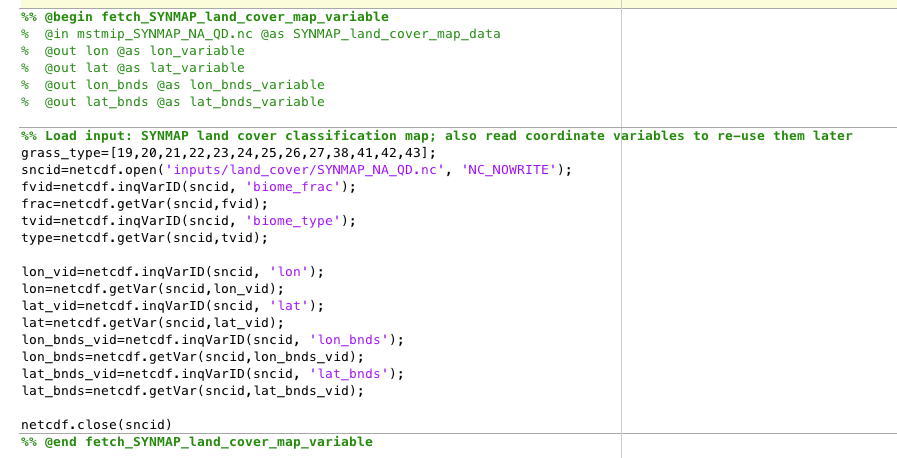
\includegraphics[width=0.5\textwidth, height=2in]{yw-annotations}
%  }
%\subfloat[Alice calls the record() function to record a run for her script \label{record-snapshot}]{%
%      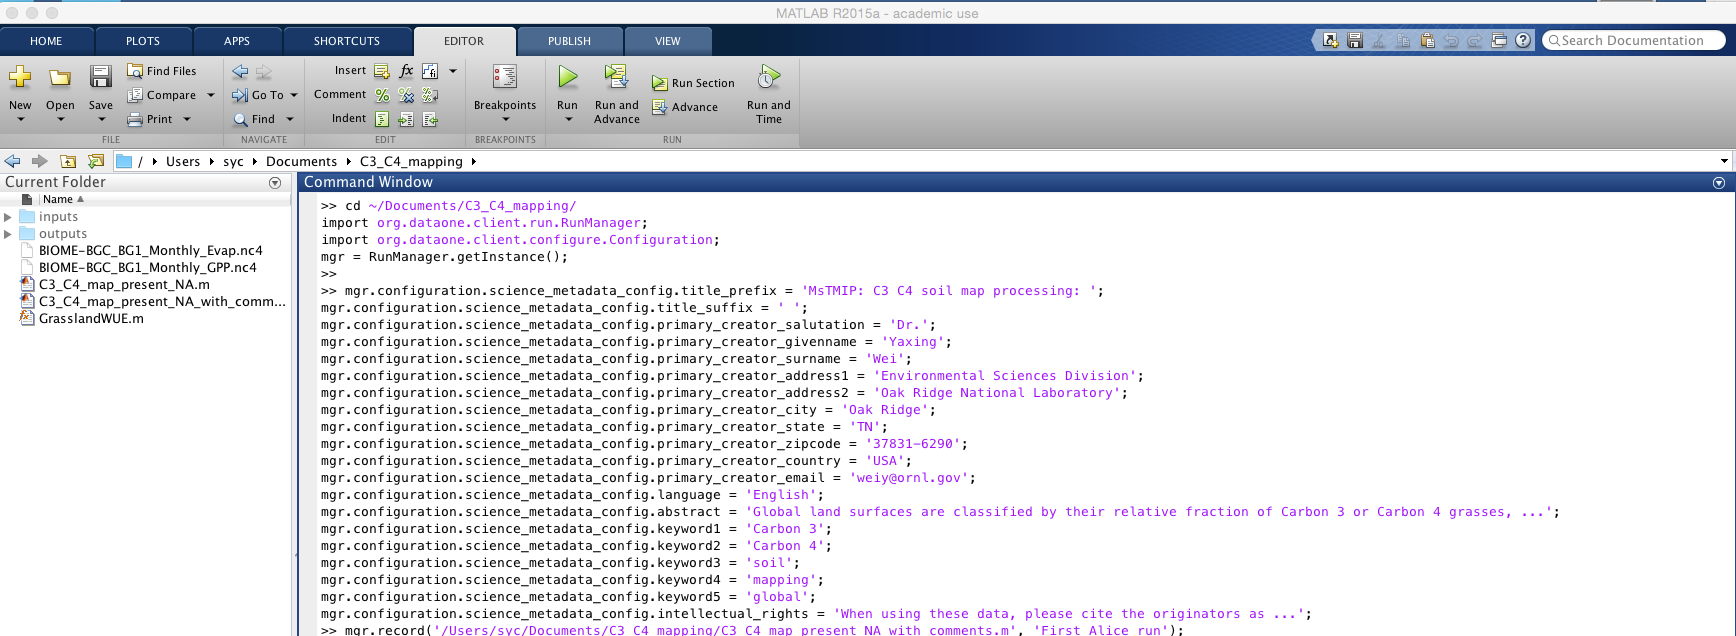
\includegraphics[width=0.5\textwidth, height=2in]{record_Alice_run}
% }
% \\
% \subfloat[Alice calls the view() function to check the recorded execution information \label{view-snapshot}]{%
%      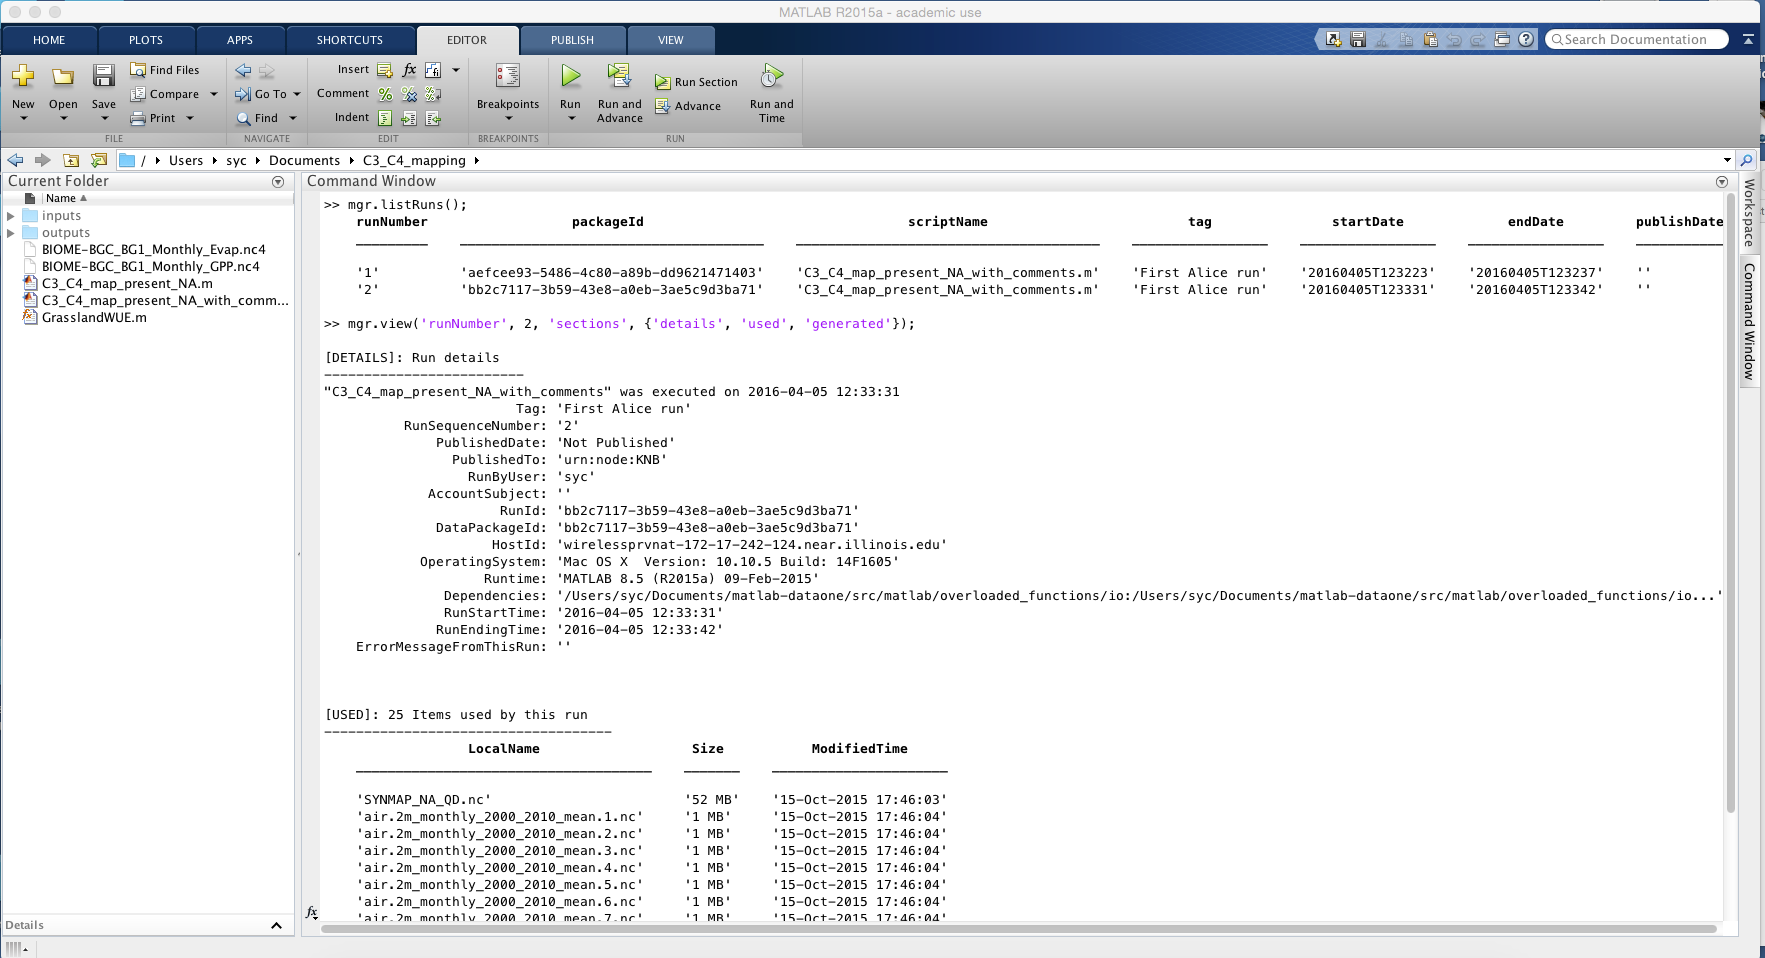
\includegraphics[width=0.5\textwidth, height=2in]{view_Alice_run}
% }
% \subfloat[Alice calls the publish() function to share her execution and data with others to DataONE network \label{publish-snapshot}]{%
%      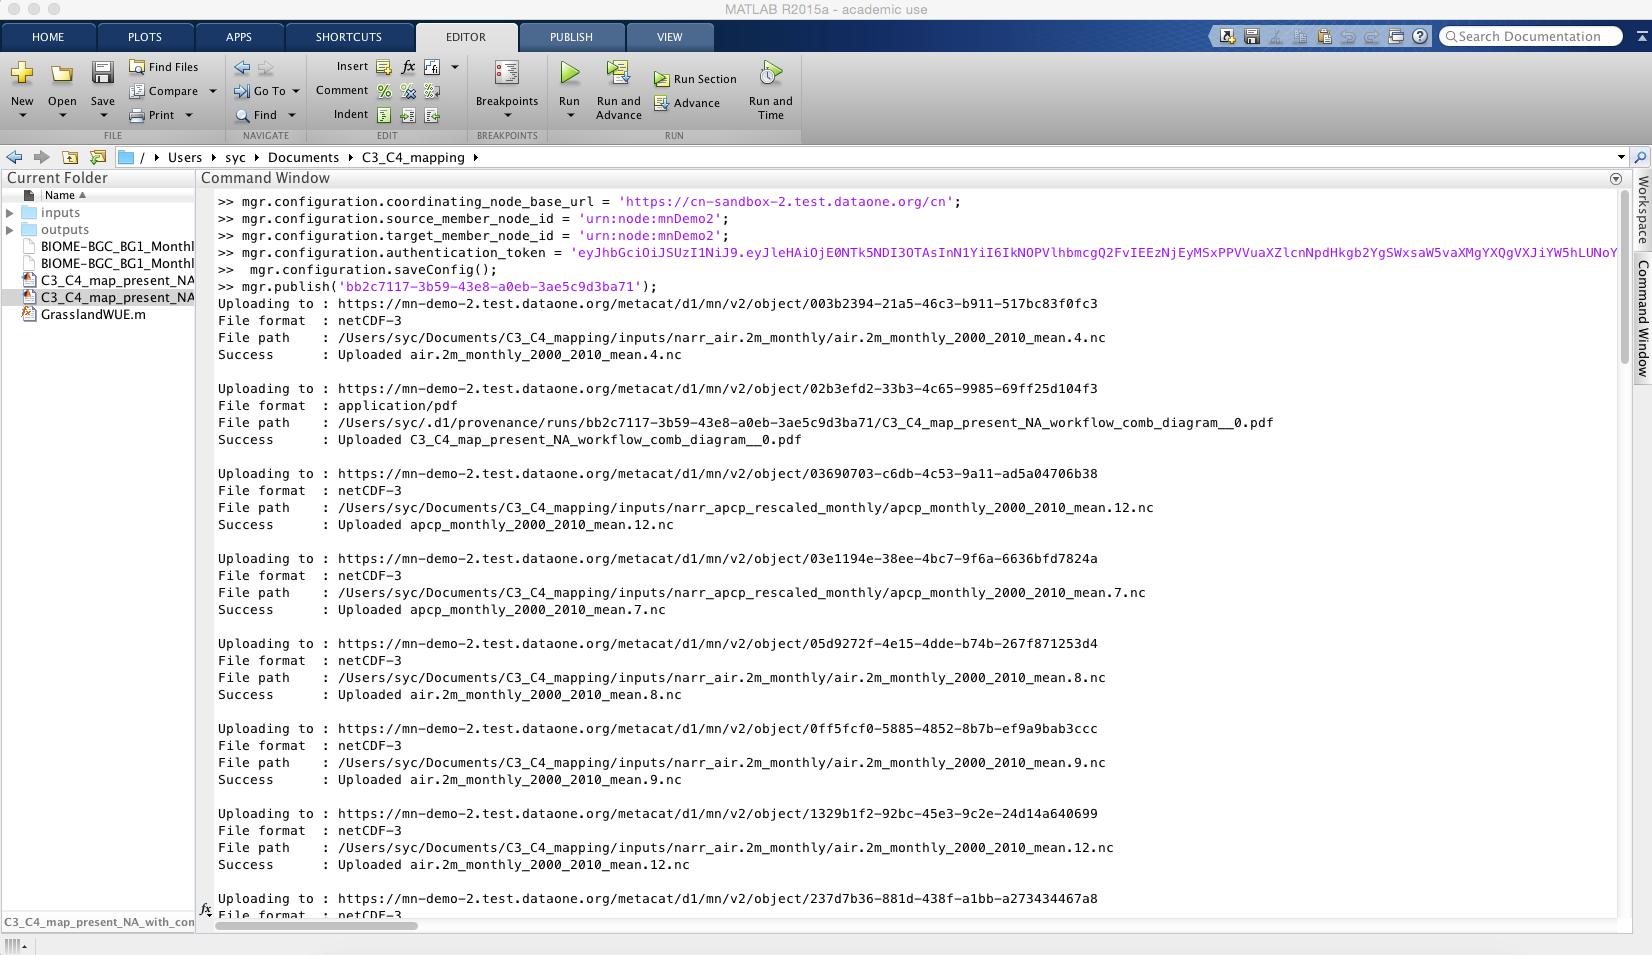
\includegraphics[width=0.5\textwidth, height=2in]{publish_Alice_run}
% }
% \caption{Snapshots when Alice uses DataONE Provenance tool to annotate her script steps, record the execution of her script, view the details for one run, and publish her run to the DataONE network.}
%\label{fig0}
%\end{figure}

\begin{figure}
\centering   
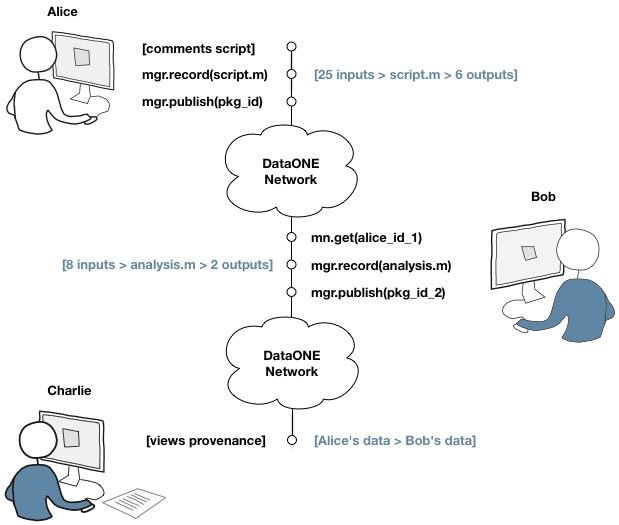
\includegraphics[width=4in, height=4in]{alice-bob-charlie-sequence}
\caption{Example use of DataONE Provenance Tool (Run Manager): (1) Alice runs her script with Run Manager to create a data package ($P_A$) and publish to DataONE network; (2) Bob downloads Alice's data, uses them in his script and creates another data package ($P_B$) using Run Manager; (3) Charlie browses data packages $P_A$ and $P_B$ and is able to navigate back to $P_A$ via $P_B$.}
\label{fig0}
\end{figure}


In Figure~\ref{fig0}, Alice has developed a script for producing Carbon3/Carbon4 soil maps. She uses YW to mark-up the code and expose the underlying workflow view (prospective provenance). Alice then ran her script using the DataONE provenance capture tool, or Run Manager, in Matlab. After a couple of runs, Alice is happy with the results and publishes them to the DataONE network. To do so, she bundles up the data results along with the runtime (retrospective) provenance captured by the DataONE Matlab provenance recorder, the script itself and its YW-generated workflow view. 

When searching DataONE for grass fraction datasets, Bob finds Alice's data package \cite{yaxing}. Bob uses outputs from Alice for his own study, which he also shares via DataONE. Since he used the unique identifiers from Alice's outputs, the provenance traces produced by Alice's and Bob's runs are naturally connected, through the nodes that carry those data identifiers. Charlie discovers Bob's data packages on DataONE and is able to navigate back to the data that Bob used, i.e., Alice's data package depicted in Figure~\ref{fig2}~\cite{Katz}\cite{data-trajectories}.


\subsection{User Bob's view: Local Run Manager View}

When Bob searches for data in DataONE and finds Alice's data and code, he uses the Matlab Toolbox to fetch the data in a way that is identifier-aware, rather than having to manually maintain the provenance information. For example, he calls the \textbf{MemberNode.get}(session, identifier) function in his analysis script because this function has provenance tracking capabilities. Then, the Toolbox downloads the data and uses the same identifier to store the data locally. Additionally, a \emph{prov:used} statement that Bob is using Alice's data is recorded. 

When Bob then calls \textbf{publish}() to upload his scripts and data, data in his package that are not present in the DataONE network will be uploaded.  When all data are within the DataONE network, their respective provenance statements are indexed on the \textbf{Coordinating Node}, and are available to be used in the web provenance display.



\subsection{User Charlie's View: DataONE Search Website}

When Charlie searches the keyword ``grass'' in the DataONE Search, two data packages are found and shown in Figure~\ref{fig1}. One data package is created by Yaxing Wei (Alice) \cite{yaxing} and the other data package is created by Christopher Schwalm (Bob) \cite{christopher}. Both data packages show that provenance information is associated with each dataset (via the icon in the search record) and can be seen at DataONE Search demo site \cite{dataone-demo}.

\begin{figure}
\centering   
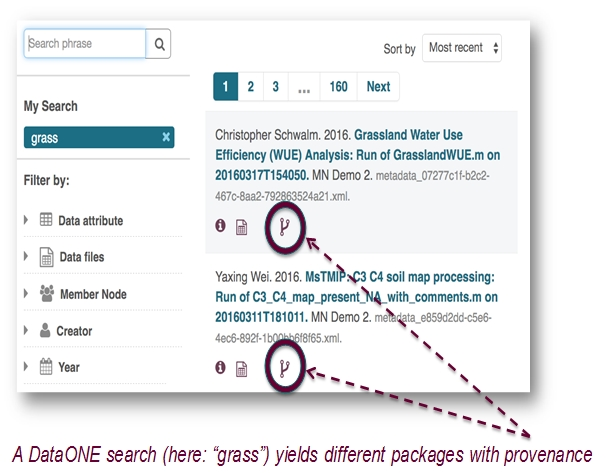
\includegraphics[width=4in, height=2in]{figure1}
\caption{The search result page for keyword  ``grass'' on a DataONE Search demo site}
\label{fig1}
\end{figure}

Prospective and retrospective provenance information can be explored from the DataONE Search site. Provenance details for any input or output in the provenance graph can be viewed by clicking on the icon shown on Figure~\ref{fig2}. DataONE Search provides human language descriptions of how data are used or generated via the script and models, and provides navigation. Figure~\ref{fig2} shows two data packages produced by the execution of Alice and Bob's workflow scripts, and the provenance lineage between these two data packages. 

Alice's data package \cite{yaxing} is shown on the top layer of Figure~\ref{fig2}, created when Alice ran her script using the DataONE provenance capture tool, or Run Manager, in Matlab. Her script (C3\_C4\_map\_present\_with\_comments.m) takes twenty-five input files and produces six outputs, which are shown on the left side and right side of Alice's data package in Figure~\ref{fig2}, respectively. The bottom three outputs in Alice's data package are the NetCDF data files that represent three different world map grids of percentage of grass types (C3 grass fraction, C4 grass fraction, and total grass fraction). In addition, a model graph is displayed at the intermediate layer \cite{yesworkflow}. Alice's workflow script used embedded YesWorkflow annotations to document her script. These annotations declare step by step how data are used and derived in the script. 


Bob's data package \cite{christopher} created by DataONE provenance tool (Run Manager) is displayed at the bottom layer. When Bob browses Alice's data package on the DataONE Search site, he decides to use three NetCDF output data produced by Alice's work in his Grassland Water Use Efficiency Analysis script (GrasslandWUE.m). From the provenance information associated with Bob's data package in Figure~\ref{fig2}, we see that it takes eight inputs, and produces two visualizations. By viewing the details for each input, we can see that three of them are the outputs produced by Alice's data package.  

In order to maintain the link between the outputs from Alice's data package to the inputs to Bob's package, Bob needs to use the same identifier in his script as Alice does. An alternative approach is that Bob creates a new identifier when he downloads Alice's data. However, the link between two data packages will be broken which has been discussed in \cite{missing-link}.  

\begin{figure}
\centering   
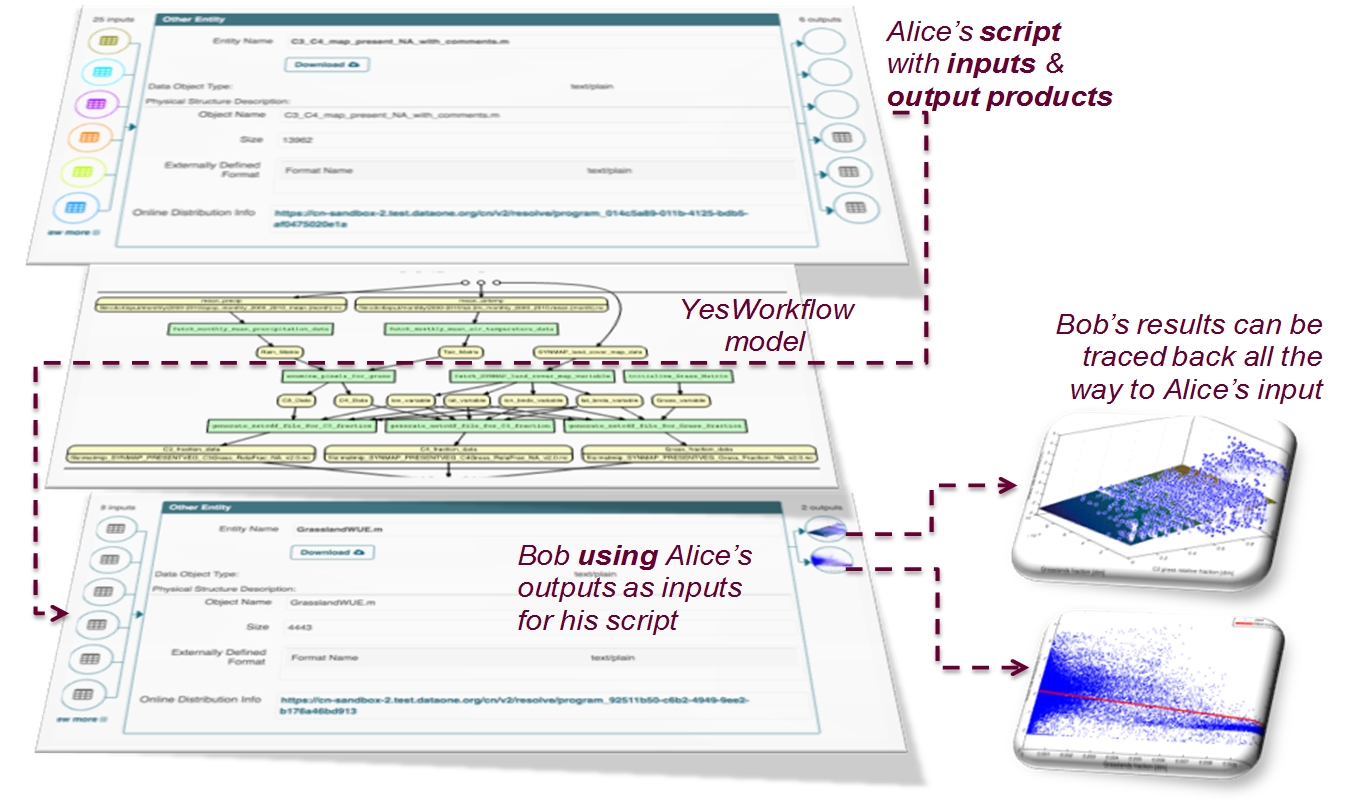
\includegraphics[width=4in, height=3in]{figure2}
\caption{User Charlie's view on DataONE Search site: (1) A combined-view YesWorkflow model for Alice's soil processing workflow script; (2) Provenance lineage between Alice's data package and Bob's data package; (3) Two visualizations produced by Bob's water use efficiency analysis script.}
\label{fig2}
\end{figure}


\section{Discussion and future work}

This paper demonstrates a notable new feature (provenance capture and search) of DataONE. DataONE has released the DataONE Search for public use in November 2015, and the R and Matlab provenance tool to the public in 2016. 

Maintaining the link between Alice's work and Bob's subsequent work is worth to be discussed. Currently Bob must use certain functions provided by DataONE to make the provenance link to Alice's work to be correctly maintained. There are other possible ways to achieve the same goal. For example,  Bob can download Alice's data and manually add the links to Alice's work back into his data package before sharing via DataONE. A \emph{prov:was\_derived\_from} statement that local data copy for Bob is derived from Alice's data is easily to be added.

Future work of the current provenance tools include: (1) solve the broken link use case; (2) support more I/O functions; (3) handle complex scenarios such as multiple runs of a script and multiple users; (4) variable-level provenance capture warrants further investigation and efforts.



\begin{thebibliography}{4}
\small

\bibitem{christopher} Christopher Schwalm's DataPackage, \url{https://search-sandbox-2.test.dataone.org/#view/metadata_07277c1f-b2c2-467c-8aa2-792863524a21.xml}

\bibitem{yaxing} YaXing Wei's DataPackage, \url{https://search-sandbox-2.test.dataone.org/#view/metadata_e859d2dd-c5e6-4ec6-892f-1b00bb6f8f65.xml}

\bibitem{dataone} Data Observation Network for Earth (DataONE), \url{https://www.dataone.org}

\bibitem{dataone-demo} DataONE Search Demo Site, \url{https://search-sandbox-2.test.dataone.org}

\bibitem{matlabdataone} Jones C., Cao Y., Slaughter P., Jones M.: Matlab DataONE Toolbox. \url{https://github.com/DataONEorg/matlab-dataone} (2016)

\bibitem{Katz} Katz, D.S. \& Smith, A.M.: Implementing Transitive Credit with JSON-LD. Journal of Open Research Software. 3(1), p.e7. (2015) 

\bibitem{yesworkflow} McPhillips T., Song T., Kolisnik T., Aulenbach S., Belhajjame K., Bocinsky R.K., Cao Y., Cheney J., Chirigati F., Dey S., Freire J., Jones C., Hanken J., Kintigh K.W., Kohler T.A., Koop D., Macklin J. A., Missier P., Schildhauer M., Schwalm C., Wei Y., Bieda M., and Ludascher B.: YesWorkflow: A User-Oriented, Language-Independent Tool for Recovering Workflow Information from Scripts. International Journal for Digital Curation, vol. 10, 298--313. (2015)

\bibitem{missing-link} Missier, P., Ludascher, B., Bowers, S., Anand, M. K., Altintas, I., Dey, S., Sarkar, A., Shrestha, B. and Goble, C.: Linking Multiple Workflow Provenance Traces for Interoperable Collaborative Science.  In: 5th Workshop on Workflows in Support of Large-Scale Science. (2010). 

\bibitem{data-trajectories} Missier, P.: Data Trajectories: Tracking Reuse of Published Data for Transitive Credit Attribution. In: 11th International Data Curation Conference. (2016). 

\bibitem{recordr} Slaughter P., Jones M., Jones C.: NCEAS recordr: Provenance tracking for R. \url{https://github.com/NCEAS/recordr} (2016)

\bibitem{oaiore} Open Archives Initiative Object Reuse and Exchange, \url{https://www.openarchives.org/ore/}







\end{thebibliography}


\end{document}
